\documentclass[12pt]{article}
\usepackage[left=1cm, right=1cm, top=2cm,bottom=1.5cm]{geometry} 

\usepackage[parfill]{parskip}
\usepackage[utf8]{inputenc}
\usepackage[T2A]{fontenc}
\usepackage[russian]{babel}
\usepackage{enumitem}
\usepackage[normalem]{ulem}
\usepackage{amsfonts, amsmath, amsthm, amssymb, mathtools}

\usepackage{fancyhdr}
\pagestyle{fancy}
\renewcommand{\headrulewidth}{1.5pt}
\renewcommand{\footrulewidth}{1pt}

\usepackage{graphicx}
\usepackage[figurename=Рис.]{caption}
\usepackage{subcaption}
\usepackage{float}

%%Наименование папки откуда забирать изображения
\graphicspath{ {./images/} }

%%Изменение формата для ввода доказательства
\renewcommand{\proofname}{$\square$  \nopunct}
\renewcommand\qedsymbol{$\blacksquare$}

\addto\captionsrussian{%
	\renewcommand{\proofname}{$\square$ \nopunct}%
}
%% Римские цифры
\newcommand{\RN}[1]{%
	\textup{\uppercase\expandafter{\romannumeral#1}}%
}


\theoremstyle{definition}
\newtheorem{defn}{Опр:}
\newtheorem{rem}{Rm:}
\newtheorem{prop}{Утв.}
\newtheorem{exrc}{Упр.}
\newtheorem{lemma}{Лемма}
\newtheorem{theorem}{Теорема}
\newtheorem{corollary}{Следствие}

\newenvironment{cusdefn}[1]
{\renewcommand\thedefn{#1}\defn}
{\enddefn}



\DeclareRobustCommand{\divby}{%
	\mathrel{\text{\vbox{\baselineskip.65ex\lineskiplimit0pt\hbox{.}\hbox{.}\hbox{.}}}}%
}


\newcommand{\smallerrel}[1]{\mathrel{\mathpalette\smallerrelaux{#1}}}
\newcommand{\smallerrelaux}[2]{\raisebox{.1ex}{\scalebox{.75}{$#1#2$}}}

\newcommand{\smallin}{\smallerrel{\in}}
\newcommand{\smallnotin}{\smallerrel{\notin}}

\begin{document}
\lhead{Математический анализ - I}
\chead{Шапошников С.В.}
\rhead{Лекция - 12}
	
\begin{corollary}\textbf{Связность прямой:} \hfill
	\begin{enumerate}[label={\arabic*)}]
		\item Числовую прямую $\mathbb{R}$ нельзя представить в виде объединения двух открытых множеств \\
		$U, V \colon U \neq \varnothing, \, V \neq \varnothing, \, U \cap V = \varnothing$;
		\item Числовую прямую $\mathbb{R}$ нельзя представить в виде объединения двух замкнутых множеств \\
		$F_1, F_2 \colon F_1  \neq \varnothing, \, F_2  \neq \varnothing, \, F_1 \cap F_2 = \varnothing$;
		\item 	Если множество одновременно замкнуто и открыто, то оно $\mathbb{R}$ или $\varnothing$;
	\end{enumerate}
\end{corollary}

\begin{proof}\hfill
	\begin{enumerate}[label={\arabic*)}]
		\item $\mathbb{R} = U \cup V, \, U \neq \varnothing, \, V \neq \varnothing, \, U \cap V = \varnothing$. $(\alpha, \beta )\subset U \colon \alpha \notin U \wedge \beta \notin U$. Хотя бы одно из $\alpha$ и $\beta$ является числом (т.е. не $\pm \infty$, иначе одно из множеств было бы пустым). Пусть, например это $\alpha$. Тогда $\alpha \notin U \Rightarrow \alpha \in V$, так как все вещественные числа либо в $U$, либо в $V$. Но $V$ - открытое множество $\Rightarrow \exists \, (\alpha - \varepsilon , \alpha + \varepsilon) \subset V, \, \varepsilon > 0$
		\begin{figure}[H]
			\centering
			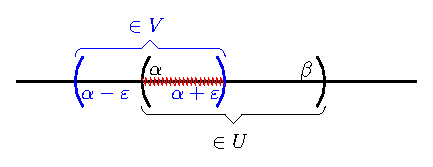
\includegraphics[width=0.4\textwidth]{12_1.eps}
			\caption{Пересечение множеств $U$ и $V$.}
			\label{12_1}
		\end{figure}
		Получаем, что интервал $V \supset (\alpha, \alpha + \varepsilon) \subset U$, но $U \cap V = \varnothing \Rightarrow$ противоречие.
		\item $\mathbb{R} = F_1 \cup F_2, \, F_1 \neq \varnothing, \, F_2 \neq \varnothing, \, F_1 \cap F_2 = \varnothing$. Тогда $F_1 = \mathbb{R} \setminus F_2 \Rightarrow F_1$ - открытое, $F_2 = \mathbb{R} \setminus F_1 \Rightarrow$ \\ $\Rightarrow F_2$ - открытое $\Rightarrow$ все свелось к пункту $1) \Rightarrow$ противоречие.
		\item Пусть $E \neq \varnothing$ и одновременно открыто и замкнуто. Тогда $\mathbb{R} \setminus E$ - открыто и замкнуто $\Rightarrow$ \\
		$\mathbb{R} = E \cup (\mathbb{R} \setminus E)$. $E$ - открыто и не пусто, $\mathbb{R} \setminus E$ - открыто $\Rightarrow \mathbb{R} \setminus E = \varnothing$ по $1) \Rightarrow \mathbb{R} = E$.
	\end{enumerate}
\end{proof}
	
\begin{defn}
	Точка $a$ - \uwave{внутренняя точка множества} $E \subset \mathbb{R}$, если существует окрестность $\mathcal{U}(a) \subset E$.
\end{defn}

\textbf{Пример}: $E$ - открыто $\Leftrightarrow$ все его точки - внутренние.
	
\begin{defn}
	Точка $a$ - \uwave{граничная точка множества} $E \subset \mathbb{R}$, если $\forall \mathcal{U}(a)$ верно $\mathcal{U}(a) \cap E \neq \varnothing \wedge \mathcal{U}(a) \cap (\mathbb{R} \setminus E)  \neq \varnothing$.
\end{defn}

\textbf{Пример}: $E = [0,1) \cup \{2\}$. Точка $\{2\}$ - не внутренняя точка: в окрестности кроме двойки ничего не лежит. 
\uline{Внутренние точки}: $(0,1)$. \uline{Граничные точки}: $\{0\} \cup \{1\} \cup \{2\}$. \uline{Предельные точки}: $[0,1]$.
	
\begin{figure}[H]
	\centering
	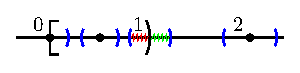
\includegraphics[width=0.35\textwidth]{12_2.eps}
	\caption{Пример классификации точек.}
	\label{12_2}
\end{figure}

\begin{defn}
	Точка $a$ - \uwave{предельная точка множества} $E \subset \mathbb{R}$, если $\forall \mathcal{U}(a), \, E \cap \mathcal{U}(a)$ - бесконечное множество. Внутренние точки - всегда предельные.
\end{defn}


\begin{theorem}
	Точка $a$ - предельная точка $E \Leftrightarrow \forall \mathcal{U}^\prime(a) = \mathcal{U}(a) \setminus \{a\}, \, \mathcal{U}^\prime(a) \cap E \neq \varnothing$.
\end{theorem}

\begin{proof}\hfill\\
	$(\Rightarrow)$ Если $a$ - предельная точка, то $\forall \mathcal{U}(a)$ множество $\mathcal{U}(a) \cap E$ - бесконечно, тогда $(\mathcal{U}(a) \cap E) \setminus \{a\} = $ $= \mathcal{U}^\prime(a) \cap E$ - бесконечно (в частности не пусто).
	
	$(\Leftarrow)$ Предположим, что $a$ - не является предельной точкой, тогда $\exists \, \mathcal{U}(a) \colon E \cap \mathcal{U}(a) = $ конечное множество. \\
	Если $E \cap \mathcal{U}(a) = \varnothing \Rightarrow E \cap \mathcal{U}^\prime(a) = \varnothing$, что невозможно. Если $E \cap \mathcal{U}(a) \neq \varnothing \Rightarrow$ пусть $x_1, \dotsc, x_N$ - элементы множества $E \cap \mathcal{U}(a) \colon x_k \neq a$. Если таких $x_k$ нет, то $(\mathcal{U}(a) \cap E) \setminus \{a\} = \varnothing \Rightarrow \mathcal{U}^\prime(a) \cap E = \varnothing$, что невозможно. Пусть такие $x_k$ есть. Возьмем $$\varepsilon = \underset{1 \leq k \leq N}{\min} \{\,|x_k -a| \,\}, \, \mathcal{U}^{\prime}_{\varepsilon}(a) = (a-\varepsilon, a + \varepsilon) \setminus \{a\}$$
	Поскольку $\varepsilon$ - минимальное расстояиние от $x_k$ до $a$, то $x_k \notin  \mathcal{U}^{\prime}_{\varepsilon}(a), \, a \notin  \mathcal{U}^{\prime}_{\varepsilon}(a) \Rightarrow  \mathcal{U}^{\prime}_{\varepsilon}(a) \cap E = \varnothing$ - противоречие.
	
		
	\begin{figure}[H]
		\centering
		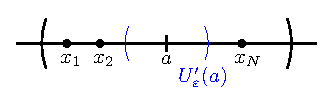
\includegraphics[width=0.35\textwidth]{12_3.eps}
		\caption{Доказательство в обратную сторону.}
		\label{12_3}
	\end{figure}
	
\end{proof}

\begin{theorem}\textbf{(Больцано)}: 
	Если $E$ - бесконечно и ограниченно, то у множества $E$ есть хотя бы одна предельная точка.	
\end{theorem}

\begin{rem}
	Множество ограниченно, если оно лежит в некотором отрезке.
\end{rem}

\begin{proof}
	Можно доказать, как теорему Больцано для подпоследовательностей. 
	
	Докажем немного по-другому пути: Так как $E$ - бесконечно, то существует последовательность $a_n$ элементов $E$ такая, что $a_n \neq a_m, n \neq m$.	
	
	Так как $E$ - ограниченно, то $\{a_n\}$ - ограниченная. По теореме Больцано для последовательностей $\exists$ подпоследовательность $a_{n_k}\! \rightarrow a$.
	Проверим, что $a$ - предельная точка $E$: по определению предела $\forall \mathcal{U}(a), \, \exists \, N \colon \forall k > N, \, a_{n_k} \in \mathcal{U}(a) \Rightarrow \mathcal{U}(a) \cap E$ - бесконечно.
\end{proof}

Разница между частичным пределом и предельной точкой: $1, 2, 1, 2, 1, 2, \dotsc$ - множество состоящее из двух элементов $\{1,2\}$. У него есть частичный предел, но нет предельной точки.

Также есть постоянные последовательности из $1$-го числа. Там также нет предельных точек.

\begin{exrc}
	Доказать, что если множество $E$ не является счетным или конечным, то у него есть предельная точка. Не предполагается, что это множество ограниченно.
\end{exrc}

\begin{theorem}
	Следующие утверждения эквивалентны:
	\begin{enumerate}[label={(\arabic*)}]
		\item Множество $E$ замкнуто;
		\item $E$ содержит все свои граничные точки;
		\item $E$ содержит все свои предельные точки;
		\item Если $a_n \in E$ и $\lim\limits_{n \to \infty} a_n = a$, то $a \in E$;	
	\end{enumerate}
\end{theorem}

\begin{proof}\hfill\\
	$(1) \Rightarrow (2)$: 
	
	\begin{figure}[H]
		\centering
		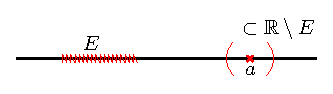
\includegraphics[width=0.35\textwidth]{12_4.eps}
		\caption{$a$ - граничная, но $a \notin E$.}
		\label{12_4}
	\end{figure}

	Если $a$ - граничная точка и $a \notin E$,  то $a \in \underbrace{\mathbb{R} \setminus E}_{\text{откр.}}$ и $\exists \, \mathcal{U}(a) \subset \mathbb{R}\setminus E$, что противоречит определению граничной точки $a$. Следовательно, либо $a$ - граничная, либо $a \in E \Rightarrow a \in E$.
	
	$(2) \Rightarrow (3)$: 
	
	\begin{figure}[H]
		\centering
		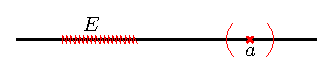
\includegraphics[width=0.35\textwidth]{12_5.eps}
		\caption{$a$ - предельная точка и $a \notin E$.}
		\label{12_5}
	\end{figure}
	
	Предположим, что $a$ - предельная точка $E$, но $a \notin E$, тогда $\forall \mathcal{U}(a), \, \mathcal{U}(a) \cap E \neq \varnothing$ (по определению предельной точки) и $\mathcal{U}(a) \cap (\mathbb{R}\setminus E) \neq \varnothing$, так как там сама точка $a \Rightarrow a$ - граничная точка, но по $(2) \, a \in E \Rightarrow$ противоречие.
	
	$(3) \Rightarrow (4)$: Пусть $a_n \to a$ и $a_n \in E$. Если $\exists \, n\colon a_n = a$, то все доказано.\\ 
	Если $\forall n, \, a_n \neq a$, то во всякой окрестности точки $a$ бесконечно много элементов $E$ или в каждой проколотой окрестности есть элемент $E$: $\forall \mathcal{U}(a), \, \exists \, N \colon \forall n > N, \, a_n \neq a \colon a_n \in \mathcal{U}(a) \Leftrightarrow a_n \in \mathcal{U}^\prime(a) \Rightarrow a$ - предельная точка $E \Rightarrow$ по $(3) \, a\in E$.
	
	$(4) \Rightarrow (1)$:
	\begin{figure}[H]
		\centering
		\includegraphics[width=0.35\textwidth]{12_6.eps}
		\caption{$a_n \to a, \, a_n \in E$.}
		\label{12_6}
	\end{figure}
	
	Пусть $a \in \mathbb{R}\setminus E$. Если во всякой окрестности $(a - \dfrac{1}{n}, a + \dfrac{1}{n})$ есть элемент $a_n \in E$, то имеется последовательность $a_n \to a$. По $(4) \, a \in E$, что невозможно $\Rightarrow \exists \, n \colon (a - \dfrac{1}{n}, a + \dfrac{1}{n}) \subset \mathbb{R} \setminus E \Rightarrow \mathbb{R} \setminus E$ - открыто $\Rightarrow$ \\
	$\Rightarrow E$ - замкнуто.
\end{proof}

\begin{exrc}
	Всякое замкнутое множество является чьим-то множеством частичных пределов.
\end{exrc}

\textbf{Пример}: множество частичных пределов последовательности - замкнуто.

\begin{proof}
	Пусть $S$ - множество частичных пределов $a_n$. Если $S = \varnothing$, то все доказано. Если $S \neq \varnothing$, то пусть $s_n \in S \colon s_n \to s$. Если $s \in S \Rightarrow$ все доказано, так как замкнутость равносильна тому, что все пределы всех сходящихся последовательностей лежат в нашем множестве.
	
	Найдем 
	$$a_{n_1} \colon |s_1 - a_{n_1}| < 1, \, n_2 > n_1 \colon |s_2 - a_{n_2}| < \frac{1}{2}, \, \dotsc , \,n_k  > n_{k-1} \colon |s_k - a_{n_k}| < \frac{1}{k}$$ 
	Не очевидно, почему можно выбирать все большие и большие номера? Частичный предел - тот к которому есть сходящаяся подпоследовательность. В сходящейся подпоследовательности будут встречаться номера сколь угодно большие. $s_2$ - частичный предел, есть сходящаяся к нему подпоследовательность, значит можно найти элементы ближе чем $\frac{1}{2}$, причем найти бесконечно много элементов, начиная с некоторого. Значит там встретится элемент с номером большим, чем $n_1$.
	
	Оценим $|s - a_{n_k}| \leq |s - s_k| + |s_k - a_{n_k}| \leq |s - s_k| + \frac{1}{k} \to 0$ по неравенству треугольника. Тогда $a_{n_k} \to s \Rightarrow$\\ $\Rightarrow s \in S \Rightarrow S$ - замкнуто по теореме выше.
\end{proof}
\end{document}